\chapter{État de l'art}

\index{état de l'art}
\index{méthode}

\section{Travaux existants}
à complèter

\section{Technologies et méthodes existantes}
\subsection{Phenomène piezoélectrique}


\subsection{Coupe du quartz}

\begin{figure}[H]
    \centering
    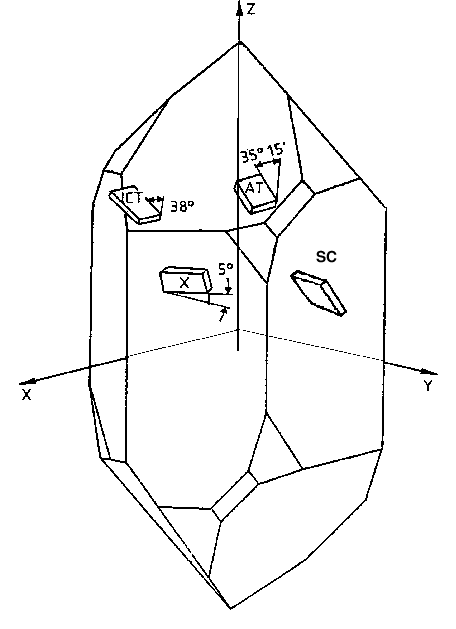
\includegraphics[width=\textwidth]{assets/figures/Orientation-of-different-cuts-in-a-natural-quartz-crystal.png}
    \caption{Différentes coupes de quartz dans un cristal naturel.}
    \label{fig:calibration plot}
\end{figure}

\begin{figure}[H]
    \centering
    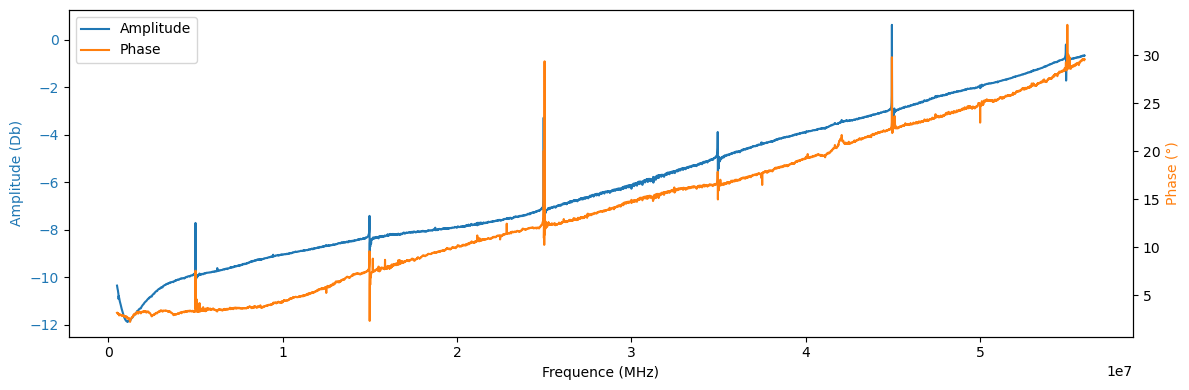
\includegraphics[width=\textwidth]{assets/figures/Calibration.png}
    \caption{Signal de calibration du capteur QCM comportant 6 pics de résonance.}
    \label{fig:calibration plot}
\end{figure}

\subsection{Capteur QCM}

\subsection{sensibilité du capteur QCM}
Le quartz à une sensibilité de a une distribution gaussienne de la masse adsorbée sur la surface du cristal.


\index{technologie}
à complèter